\documentclass[11pt,a4paper]{exam}
\printanswers % pour imprimer les réponses (corrigé)
%\noprintanswers % Pour ne pas imprimer les réponses (énoncé) - et en plus on n'en a pas ici
\addpoints % Pour compter les points
\usepackage[utf8]{inputenc}

\usepackage[margin=1in]{geometry}
\usepackage{amsmath,amssymb}
\usepackage{multicol}
\usepackage{graphicx}
\usepackage{setspace}
\usepackage{dashundergaps}

\newcommand{\class}{SNT 2\textsuperscript{nde}8}
\newcommand{\examnum}{Interrogation \#1}
\newcommand{\examdate}{25/09/2023}
\newcommand{\timelimit}{10 Minutes}
\newcommand{\lycee}{Lycée Fustel de Coulanges}

\pagestyle{head}
\firstpageheader{}{}{}
\runningheader{\class}{\examnum\ - Page \thepage\ / \numpages}{\examdate}
\runningheadrule


\begin{document}
	\noindent
	\begin{spacing}{1,5}
		\noindent
		\begin{tabular*}{\textwidth}{l @{\extracolsep{\fill}} l @{\extracolsep{6pt}} l}
			\textbf{\class} & \textbf{Nom:} & \makebox[3in]{\hrulefill}\\
			\textbf{\lycee} &&\\
			\textbf{\examnum, \examdate} &&\\
			\textbf{Durée: \timelimit} &&\\
		\end{tabular*}\\
	\end{spacing}
	
	\noindent
	\rule[1ex]{\textwidth}{2pt}
	
	\noindent
	Cette interrogation comporte \numquestions\ questions; elle sera notée sur \numpoints\ points.\\
	
	\noindent
	\rule[3ex]{\textwidth}{2pt}
	
	\begin{spacing}{1,2}
		\begin{questions} % DEBUT DE L'EXAMEN
			
			% #1 - tableau - OK
			\question Considérez le tableau suivant:
			\\
			\\
			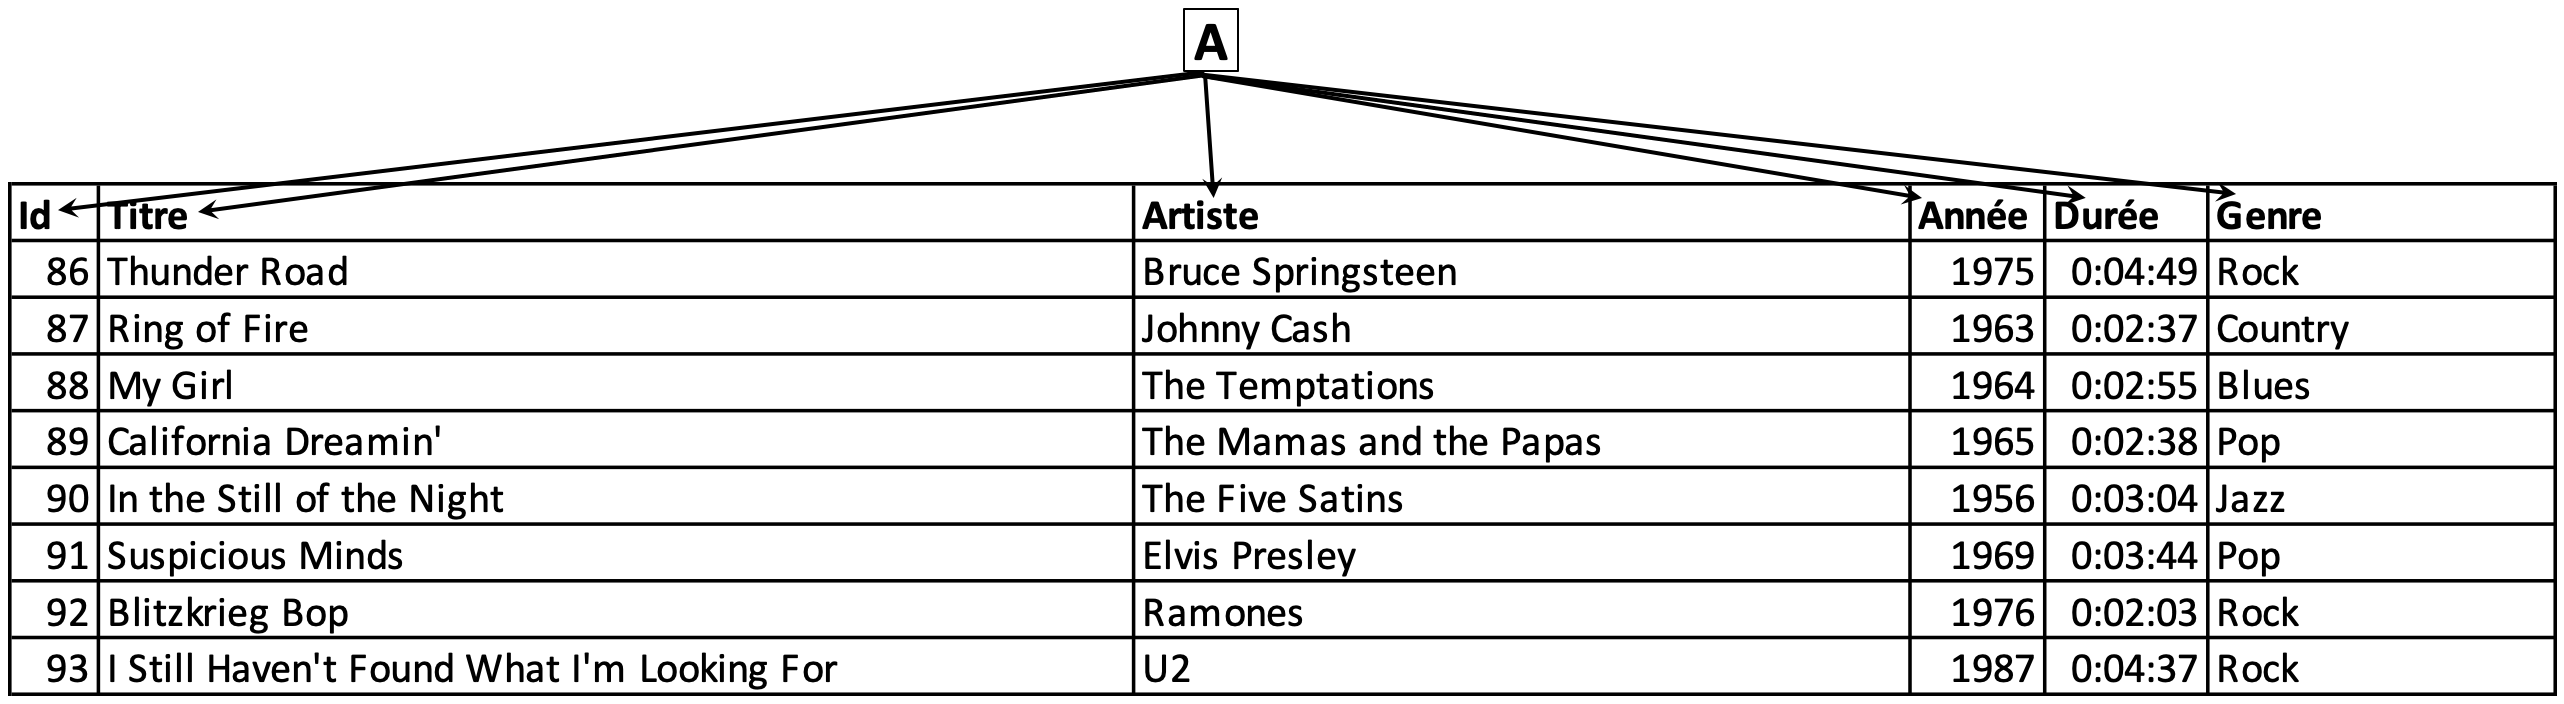
\includegraphics[width=\textwidth]{Tableau.png}
			\begin{parts}
				\part Vocabulaire des données structurées:
				\begin{subparts}
					\subpart[1] Comment appelle-t-on les  titres de colonnes (repère "A")?
					\begin{solution}
						Les en-têtes de colonnes sont appelés des \textbf{descripteurs}.
					\end{solution}
%					\makeemptybox{1,3cm}
%					\setlength\fillinlinelength{6cm}
					\subpart[1] Compléter:\\
					\\
					\textit{"Jazz" est la valeur de l'\fillin\
						"Genre" du morceau intitulé "In the Still of the Night"}
					\begin{solution}
						\textbf{attribut}.
					\end{solution}
				\end{subparts}
				\part[1] Si on appliquait à ce tableau, comme on l'a fait en TP, un filtre sur le genre
				"Rock", quelle serait le nom du deuxième artiste à apparaître dans la liste
				\textit{(sans compter la ligne des titres de colonnes)}?
%				\makeemptybox{1,3cm}
				\begin{solution}
					L'artiste en deuxième position serait \textbf{Ramones}.
				\end{solution}
				\part[1]Quelle\textit{(s)} colonne\textit{(s)} permet\textit{(tent)} d'identifier de manière unique un morceau?
%				\makeemptybox{1,3cm}
				\begin{solution}
					Plusieurs solutions ici: la plus simple, \textbf{\{Id\}} (c'est la raison d'être de cette colonne); on pouvait aussi dire \textbf{\{Artiste, Titre\}} (en partant du principe qu'un artiste n'écrit pas plusieurs chansons ayant le même titre).
				\end{solution}
			\end{parts}
			\addpoints
			
			\newpage
			
			% 2 - Métadonnées - OK
			\question[1] Pour vous, qu'est-ce qu'une "métadonnée" d'un fichier image (en une phrase) ?
%			\makeemptybox{2,6cm}
			\begin{solution}
				Une métadonnée est une donnée qui décrit ou donne des informations sur une autre donnée --- en l'occurence sur le fichier image, sans que l'information soit visible dans l'image elle-même; il peut s'agir par exemple de la date de prise de vue, du modèle de téléphone ou d'appareil photo utilisé, des coordonnées GPS de l'endroit où la prise de vue a été effectuée...
			\end{solution}
			
			% #3 - format CSV - OK
			\question[1] Parmi les formats de fichier suivants lequel a été conçu
			pour être lu par un tableur (comme Excel ou LibreOffice Calc)?
			\begin{checkboxes}
				\correctchoice CSV
				\choice JSON
				\choice XML
				\choice DOCX
				\choice HTML
			\end{checkboxes}
			\addpoints
			
			% #4 - données personnelles - OK
			\question[2] Parmi les éléments suivants le\textit{(s)}quelle\textit{(s)}
			est \textit{/ sont}, selon vous, des données personnelles (cocher les bonnes réponses)?
			\addpoints
			\begin{checkboxes}
				\correctchoice Nom
				\choice Âge
				\choice Nombre de likes d'une vidéo YouTube
				\correctchoice Adresse IP de l'ordinateur de la maison
				\choice Photo de la Tour Eiffel
				\correctchoice Photo de famille
				\choice Adresse IP de l'imprimante d'une entreprise
				\correctchoice Localisation d'un smartphone
				\correctchoice Numéro de sécurité sociale
				\choice Nombre d'employés dans une mairie
				
				\choice Données médicales anonymées (donc sans moyen d'identifier la personne concernée)
			\end{checkboxes}
			
			% #5 - Vrai / Faux
			\question[2] Vrai ou faux? Cochez la ou les propositions exactes dans la liste ci-dessous.
			\begin{checkboxes}
				\choice Toute information que l'on refuse de partager est une donnée personnelle.
				\choice Le format JSON est un format d'image.
				\correctchoice Une donnée personnelle en est une qui permet d'identifier une personne
				physique \textemdash\ directement ou indirectement.
				\correctchoice L’adresse d’une personne reste une donnée personnelle même si elle
				a été donnée volontairement (sur un site web par exemple).
			\end{checkboxes}
			
			
		\end{questions}
	\end{spacing}
	
\end{document}
